% (The MIT License)
%
% Copyright (c) 2023-2024 Yegor Bugayenko
%
% Permission is hereby granted, free of charge, to any person obtaining a copy
% of this software and associated documentation files (the 'Software'), to deal
% in the Software without restriction, including without limitation the rights
% to use, copy, modify, merge, publish, distribute, sublicense, and/or sell
% copies of the Software, and to permit persons to whom the Software is
% furnished to do so, subject to the following conditions:
%
% The above copyright notice and this permission notice shall be included in all
% copies or substantial portions of the Software.
%
% THE SOFTWARE IS PROVIDED 'AS IS', WITHOUT WARRANTY OF ANY KIND, EXPRESS OR
% IMPLIED, INCLUDING BUT NOT LIMITED TO THE WARRANTIES OF MERCHANTABILITY,
% FITNESS FOR A PARTICULAR PURPOSE AND NONINFRINGEMENT. IN NO EVENT SHALL THE
% AUTHORS OR COPYRIGHT HOLDERS BE LIABLE FOR ANY CLAIM, DAMAGES OR OTHER
% LIABILITY, WHETHER IN AN ACTION OF CONTRACT, TORT OR OTHERWISE, ARISING FROM,
% OUT OF OR IN CONNECTION WITH THE SOFTWARE OR THE USE OR OTHER DEALINGS IN THE
% SOFTWARE.

\documentclass{article}
\usepackage{../sqm}
\newcommand*\thetitle{Lines of Code (LoC)}
\begin{document}

\plush{\sqmTitlePage{1}{q9Gr2xguP5I}}

\qte
  {lionel-deimel}
  {One of the most overlooked programming skills is the ability to \ul{read} a program, an activity the programmer is called upon to do with surprising \ul{frequency}.}
  {deimel1985uses}

\qte
  {darrell-raymond}
  {Whatever approach is used, it is clear that a central activity in software maintenance is \ul{reading}. In maintenance, the main role of source code is not as a compilable entity, but as a human-readable statement of the intent and mechanism of the program.}
  {raymond1991reading}

\qte
  {shari-lawrence-pfleeger}
  {It's not enough to make claims about your software; you must support your claims with \ul{measurable evidence}.}
  {pfleeger2008software}

\thought{Everybody wants higher \ul{quality of code}, but nobody knows how to measure it.}

\thought{Code \ul{maintainability}, probably, is the ultimate objective of increasing the quality of source code.}

\thought{Code \ul{size} makes the biggest negative impact on code maintainability.}

\qte
  {edsger-dijkstra}
  {It has been suggested that there is some law of nature telling us that the amount of intellectual effort needed grows with the \ul{square} of program \ul{length}. But, thank goodness, no one has been able to prove this law. And this is because it \ul{need not be true}.}
  {dijkstra1972humble}

\qte
  {steve-mcconnell}
  {Studies have found that larger routines are more \ul{error-prone} than smaller ones. Keeping routines short helps reduce errors and makes the code easier to maintain.}
  {mcconnell2004code}

\qte
  {robert-martin}
  {The first rule of functions is that they should be \ul{small}. The second rule of functions is that they should be even \ul{smaller} than that.}
  {martin2008clean}

\thought{It \ul{may} be wrong to measure productivity of a programmer by counting lines of code, but for the quality of code the LoC metric is a perfect indicator.}

\plush{
  \pptBanner{\texttt{cloc.pl}}
  \pptPic{.65}{cloc.png}\par
  \url{https://github.com/AlDanial/cloc}}

\thought{Instead of counting lines, it may be more reasonable to count NCSS (Non Commenting Source Statements), but not always.}

\pptBanner{LoC vs NCSS}
\begin{multicols}{2}
{\small\begin{ffcode}
#!/bin/bash
set -e

# Simple intro:
printf "Hello, %s!
  Your balance is %d." \
  "${name}" \
  "$(psql 'SELECT balance
    FROM user WHERE id = 42')"
\end{ffcode}
}
\par\columnbreak\par
Lines of Code = ?
\par
NCSS = ?
\end{multicols}
\plush{}

\thought{There are \href{https://www.linux.com/news/linux-in-2020-27-8-million-lines-of-code-in-the-kernel-1-3-million-in-systemd/}{27.8M} lines of C code in Linux kernel. What does it tell us?}

\plush{
  \pptBanner{Largest Open Source Projects}
  \begin{multicols}{2}
  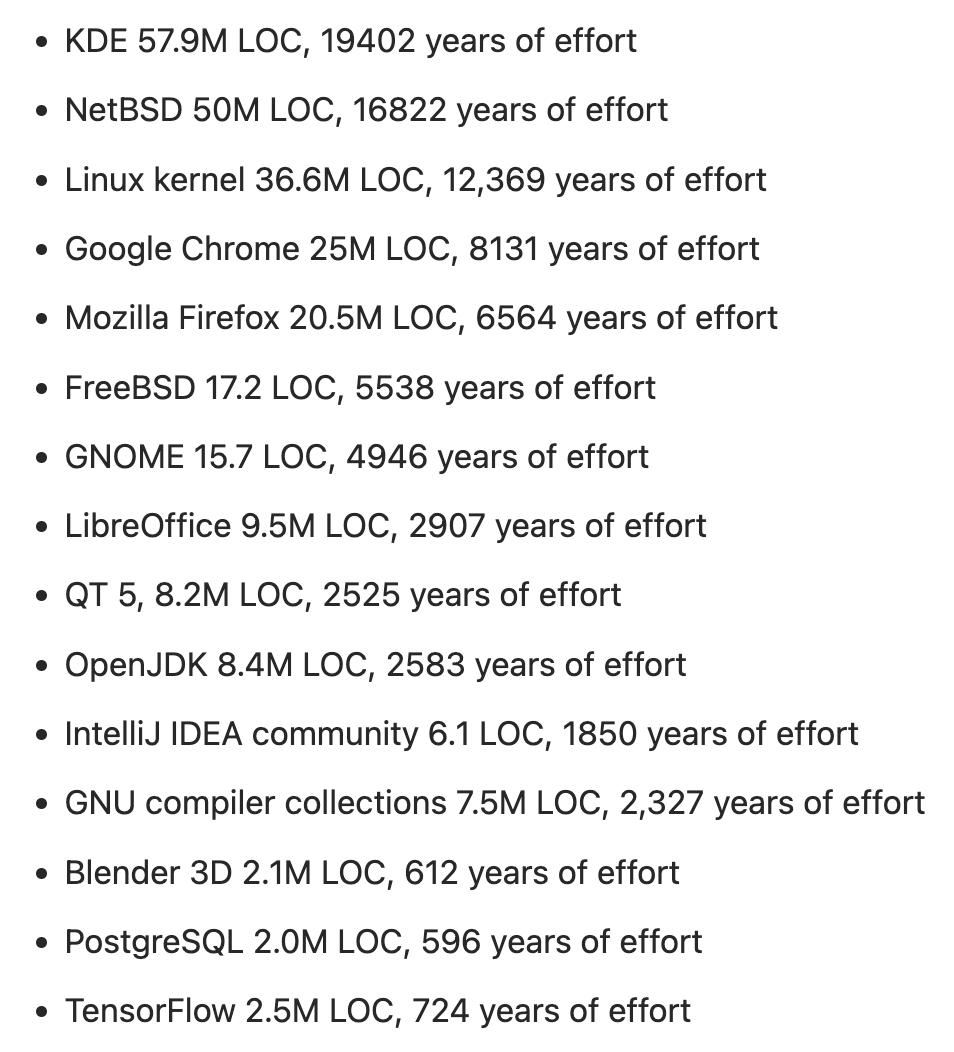
\includegraphics[width=.8\linewidth]{largest.png}\par
  {\scriptsize Found it on \href{https://www.quora.com/What-are-some-open-source-projects-with-the-largest-complexity-by-lines-of-code-or-developer-effort/answer/Felix-Zaslavskiy}{Quora}.\par}
  \par\columnbreak\par
  \tbd{what}
  \end{multicols}}

\thought{In 2011, Uncle Bob \href{https://softwareengineering.stackexchange.com/questions/66523}{suggested} that 200 lines per Java class is a good guideline to stay below.}

\thought{Java is \href{http://jameshfisher.github.io/languageredundancy/}{two times} more verbose than Ruby. Does it mean the quality of an average Ruby code is higher?}

\end{document}
